\documentclass[sigconf]{acmart}
\settopmatter{printacmref=false}
\renewcommand\footnotetextcopyrightpermission[1]{}

\usepackage{graphicx}
\graphicspath{ {./Experiment Results/} }

\usepackage[backend=bibtex]{biblatex}
\addbibresource{References.bib}

\begin{document}
    \title{Ant Colony Optimisation for the Bin Packing Problem}
    \author{710018541}
    \maketitle
    
    \section{Literature Review}
        In the early 1990s, the development of metaheuristic approaches provided new ways to tackle complex optimisation problems that were previously difficult to solve. One of the most innovative techniques to emerge was Ant Colony Optimization (ACO), inspired by the behaviour of ant colonies, which efficiently find optimal solutions to complex problems through simple, decentralised processes. ACO has since been successfully applied to various challenges, including improving the efficiency of RFID antennas\cite{4426906}, optimising vehicle routing problems\cite{Emilio2004AntCO}, and as we will see here to the Bin Packing Problem.\newline

        The Bin Packing Problem, which we will be solving using our implementation of ACO, is a general problem-solving challenge that takes multiple different forms with the same underlying principle. Some focus on minimising the number of bins used to store the items such as that outlined in Towards Bin Packing (preliminary problem survey, models with multi-set estimates)\cite{Levin2016TowardsBP}. Others like ours focus on some ideal distribution of items (in our case the goal distribution will be that which minimises the difference in weights between the heaviest and lightest bins).\newline

        Focusing on ACO it is important to have a clear understanding of the basic approach we will be taking, which will be similar to that outlined in Marco Dorigo’s paper on Ant Algorithms for Discrete Optimization\cite{10.1162/106454699568728}. Firstly we must find a way of representing our solution space in a representation traversable by our ants, this typically takes the form of a graph. ACO then breaks down the optimisation of the problem into three steps that are iterated until some termination criteria is reached; traversing the graph, evaporating pheromone, and setting pheromone.\newline
        
        Traversing of the graph by ants is done in a probabilistic manner according to the amount of pheromone present on each path. Once an ant has traversed a path, all pheromone on all paths will be evaporated by some evaporation rate e. Lastly each ant will add its own pheromone to the path according to the fitness of the solution explored (Note in our implementation we will be adding pheromone first and then evaporating as per the coursework specification).\newline

        The ACO approach for solving the Bin Packing Problem has been identified as an effective method, yet there are various other nature inspired methods that also work and in some cases outperform the ACO method, such as Particle Swarm Optimisation (PSO) introduced in 1995\cite{Eberhart1995ANO} or Genetic Algorithms (GA) introduced in 1975\cite{holland1992adaptation}.\newline
        
        Similarly to ACO, PSO is a nature-based metaheuristic based on the social flock behaviours of birds and fish and relies on the sharing of knowledge of successful solutions (allocations of items to bins) between individuals in the flock. Each individual has an initial “position” and “velocity”, corresponding to a candidate solution and the tendency to move towards better solutions respectively. This movement is determined through the particle’s current velocity, its best “known” position and the best known solution in the flock (the global best solution found), enabling the distribution of knowledge of successful paths.\newline

        The GA approach on the other hand relies on the evolution of a variety of candidate solutions through genetic operators, including selection, crossover and mutation, which provide the algorithm the ability to explore a wide solution space. The GA approach to the BPP relies on representing candidate solutions as "chromosomes" which can be altered through the aforementioned genetic operators. Advantages of GA is their ability to effectively explore broad solution spaces, however this may come at the cost of slower convergence than ACO or PSO.\newline
        
    \section{Description of Results}
        \subsection{Experimental Setup}
            As part of any experiment it essential to have a clear idea of what the we are measuring and comparing, and how the experimental setup will affect these results. To this end, we have outlined our approach below along with reasoning for many of the decisions taken. We will commence by outlining our experiment's measurements, experimental variables, and control variables. 
            
            We will be running our implementation on two variations of the bin packing problem. These two experiments will have different setups as follows
            \begin{itemize}
                \item \textbf{BPP1} - Number of bins (b) = 10, weight of item n is n
                \item \textbf{BPP2} - Number of bins (b) = 50, weight of item n is $n^2/2$\newline
            \end{itemize}

            To assess the performance of each experimental run, we will measure:
            \begin{itemize}
                \item \textbf{Best solution fitness over time} - observes the algorithm’s peak performance in each iteration.
                \item \textbf{Average solution fitness over time} - indicates overall population performance and algorithm stability.
                \item \textbf{Standard deviation of fitness over time} - provides insight into population diversity, showing how converged or exploratory the population is over time.
            \end{itemize}
            
            Each of these metrics will be averaged across multiple trials for statistical robustness.\newline
            
            Our experimental variables which we will alter throughout:
            \begin{itemize}
                \item Ant population
                \item Evaporation rate\newline
            \end{itemize}

            And lastly our control variables which we wish to keep consistent throughout:
            \begin{itemize}
                \item Initial pheromone matrix
                \item Item choice given the same probabilities in time\newline
            \end{itemize}

            To ensure consistency, we will seed random functions (random and numpy.random) so that comparable trials yield consistent initial conditions. This seeding approach ensures that:
            \begin{itemize}
                \item The initial pheromone matrix (generated using random.uniform) is identical across comparable trials, enabling fair comparison.
                \item Two ants arriving at the same decision point (i.e. choosing which bin to assign to a given item) under identical conditions will make the same choice, enhancing the experiment’s repeatability and consistency.\newline
            \end{itemize}

            In cases where an optimal solution is achieved (i.e. the weight difference between the heaviest and lightest bins is zero), we handle this edge case by setting all other paths' pheromone values to zero while setting the selected optimal path’s pheromone value to one. This adjustment allows the experiment to proceed, with ants exclusively choosing the optimal path for the remainder of the run.\newline

        \subsection{Experimental Execution}
            Please see attached copy of implementation code.
            
        \subsection{Experimental Results}
            From the results generated in the experiment described above we were able to plot the following charts, enabling us to compare the performance of our implementation of ACO for the BPP with various different experimental variable configurations. This was done for both experimental setups described in the project specification.\newline

            \subsubsection{BPP1 Experiment Results:\newline}
                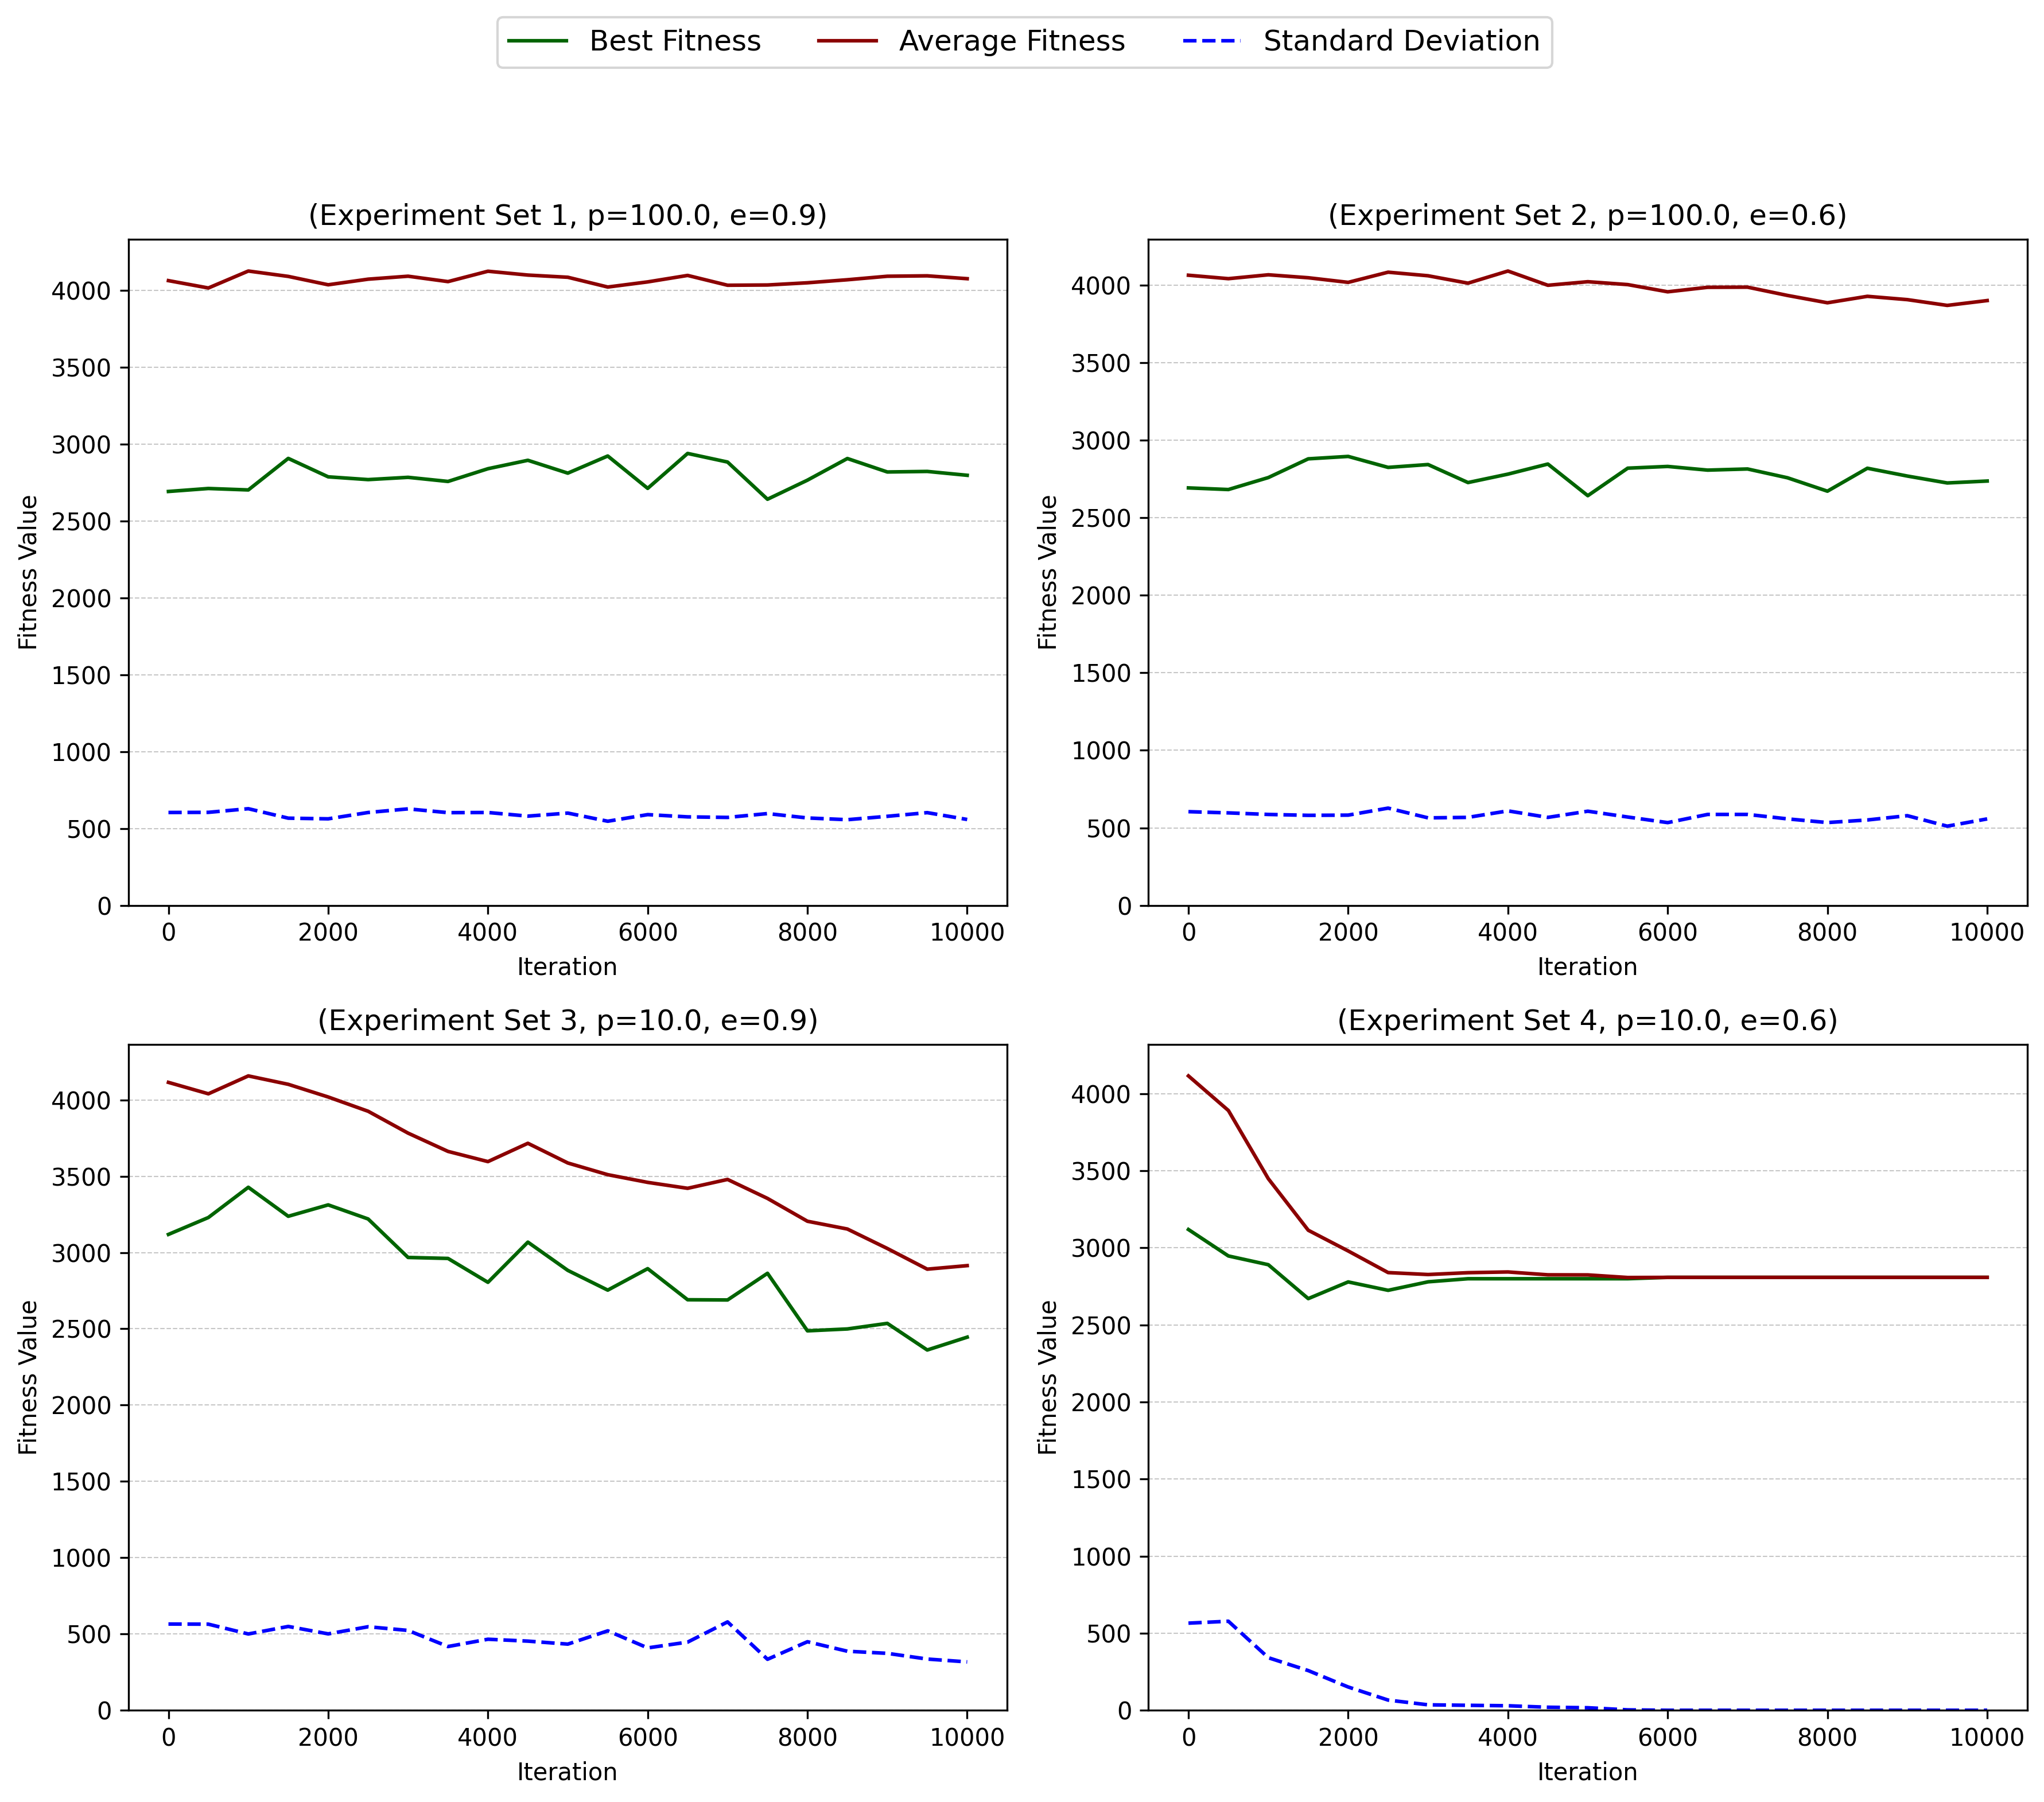
\includegraphics[scale=0.3]{Association for Computing Machinery (ACM) - SIG Proceedings Template/Experiment_Results/Experiment_BBP1_Metrics.png}

            In the charts above we can observe the results for our ACO implementation on the BPP1 experiment setup. The four charts indicate the results with different experimental variables highlighting how they affect the execution of the ACO implementation. Reading left-to-right we observe the results from Experiment Set 1, with p=100 e=0.9, Experiment Set 2, with p=100 e=0.6, Experiment Set 3, with p=10 e=0.9, Experiment Set 4, with p=10 e=0.6.

            \subsubsection{BPP2 Experiment Results:\newline}
                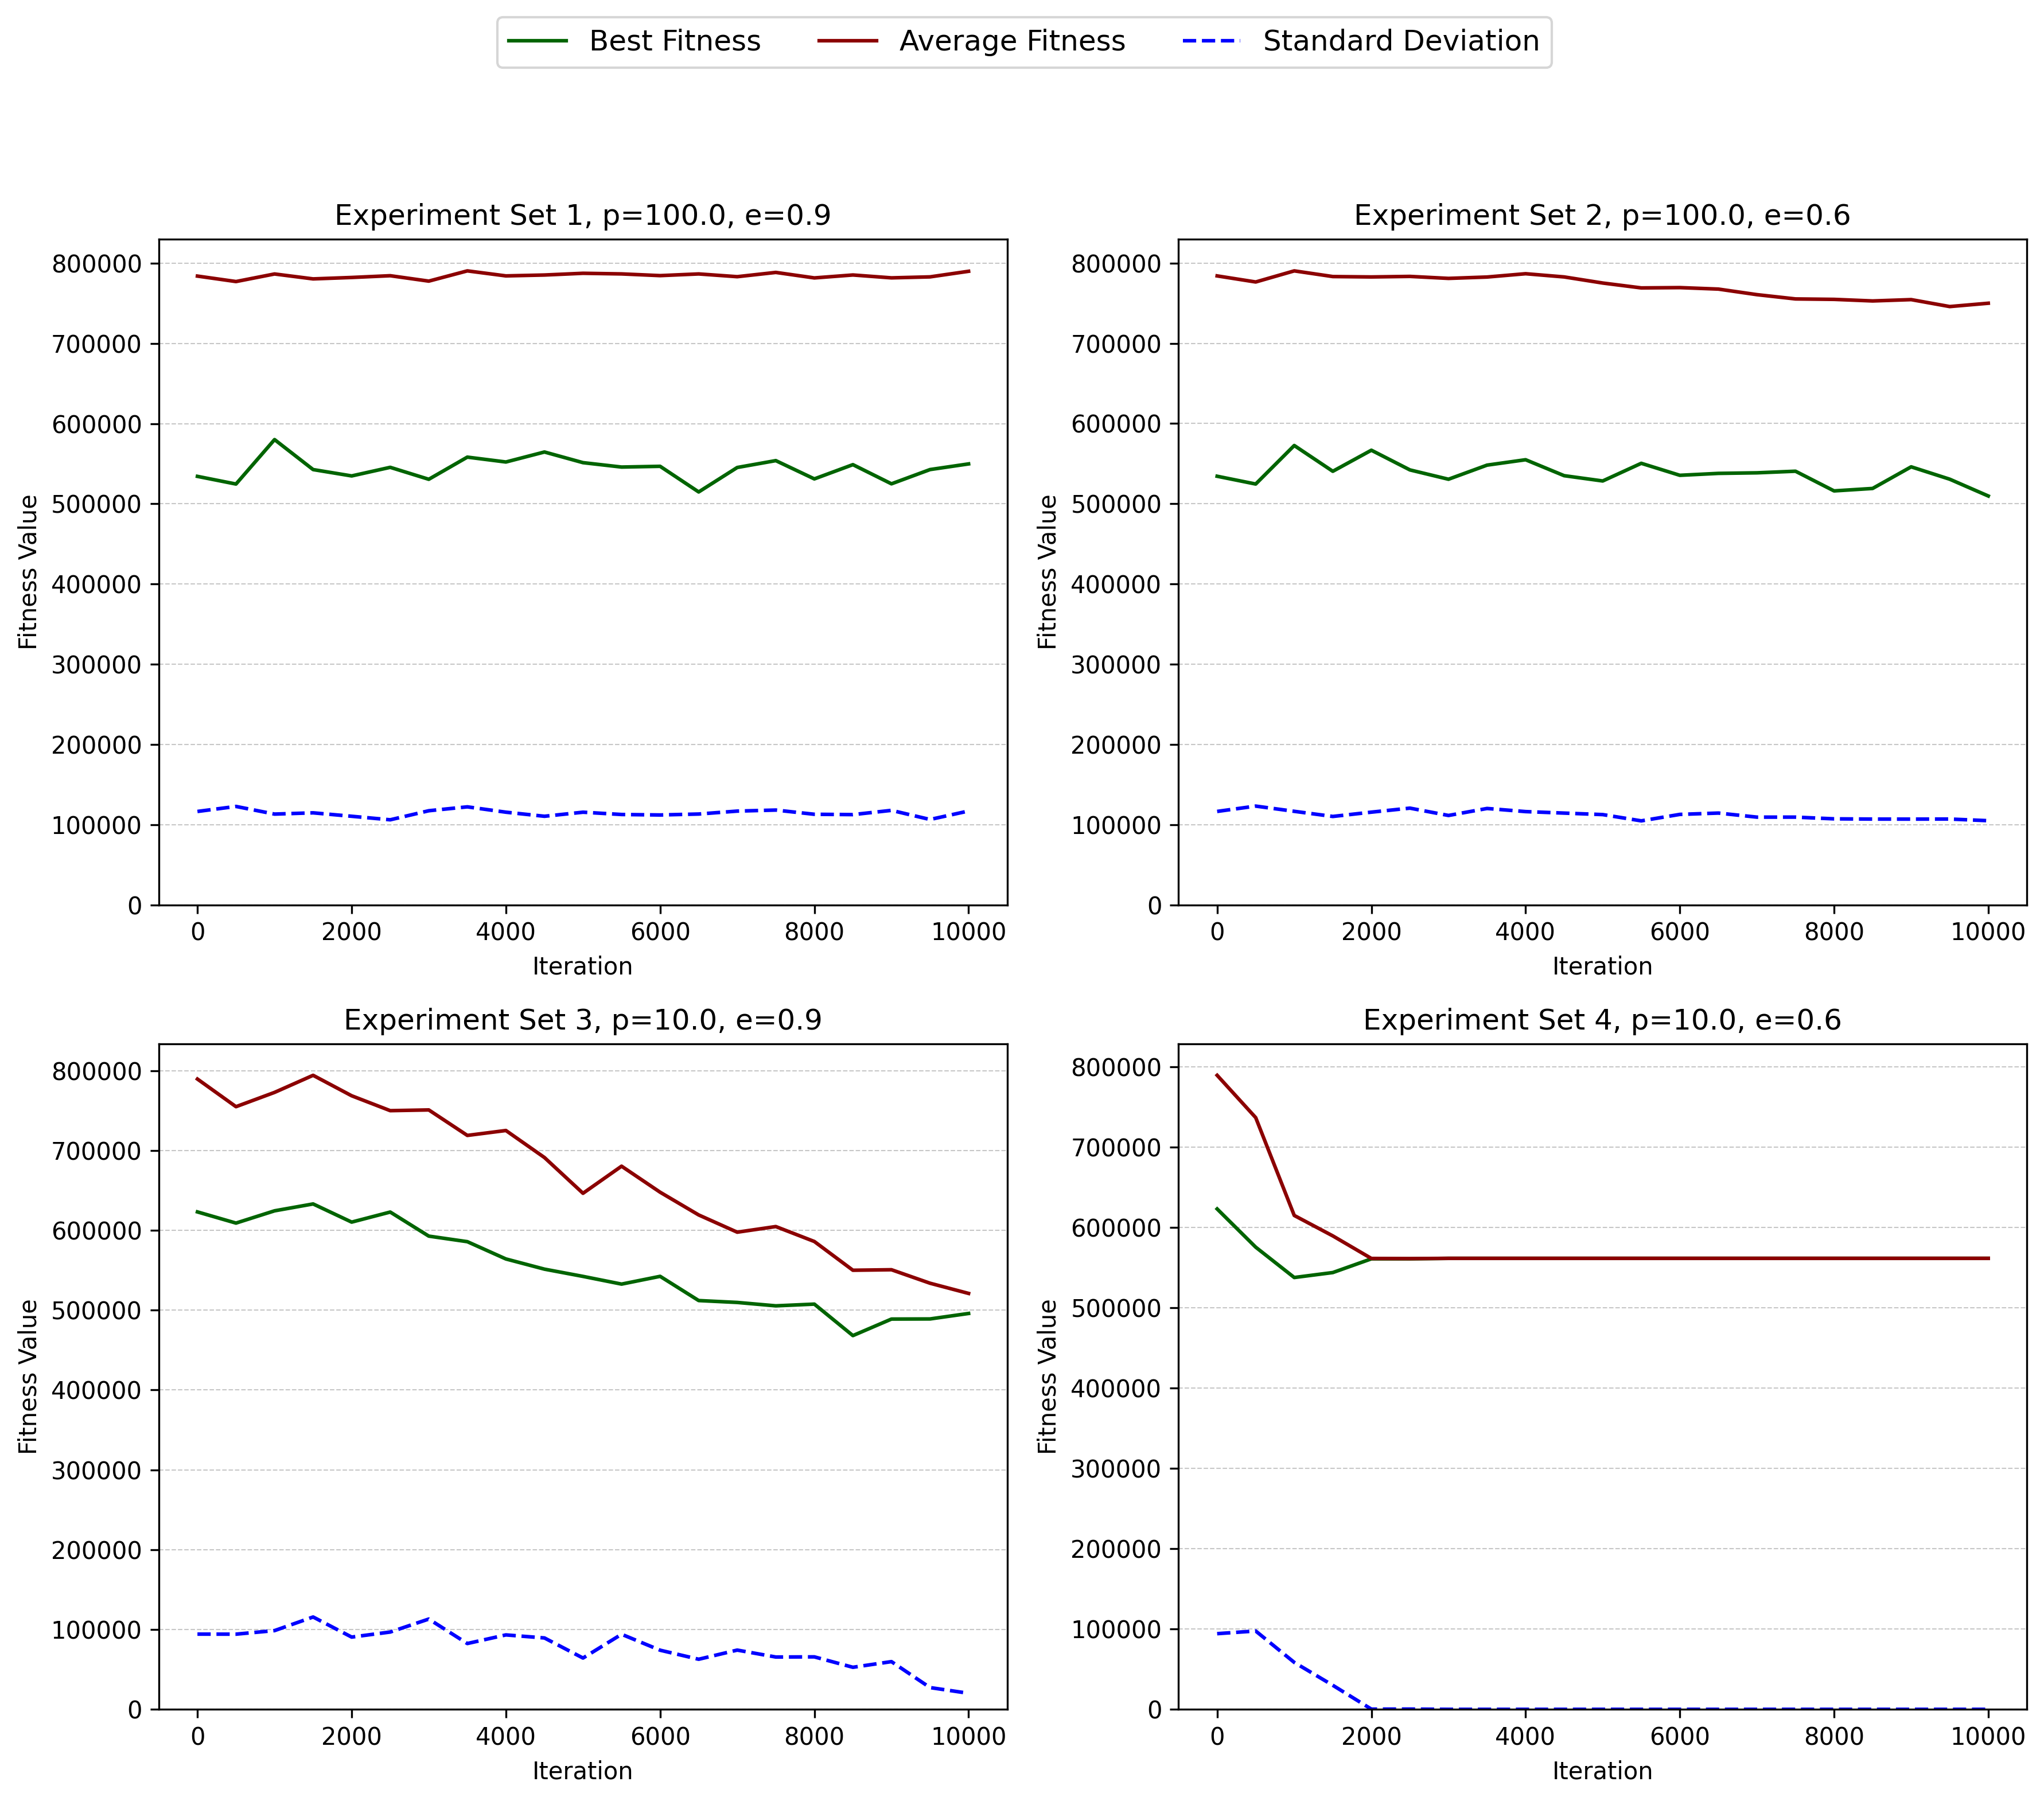
\includegraphics[scale=0.3]{Association for Computing Machinery (ACM) - SIG Proceedings Template/Experiment_Results/Experiment_BBP2_Metrics.png}

            Similarly to the results from BPP1, here we can observe the results from BPP2 with the same layout left-to-right in terms of experimental variables sets.\newline

            Importantly, in all 8 charts above, we have plotted the best fitness of the paths in green, the average fitness of the paths selected by ants in red, and lastly the standard deviation of the paths selected by ants in dashed blue. These results are based on samples taken every 500 fitness evaluations (various different sample frequencies were taking but with this frequency we manage to capture the general shape while not overburdening our implementation).\newline

            As can be see from the charts above, the trends of all three lines remain broadly consistent between corresponding experiment sets from BPP1 and BPP2. The trends for the three curves are as follows:

            \begin{itemize}
                \item Experiment Set 1:
                \begin{itemize}
                    \item Best Fitness - Fluctuating with a flat trend throughout experiment
                    \item Average Fitness - Smooth with a flat trend throughout experiment.
                    \item Standard Deviation - Smooth and flat throughout experiment.\newline
                \end{itemize}
                \item Experiment Set 2:
                \begin{itemize}
                    \item Best Fitness - Fluctuating with a very slight downward trend throughout experiment.
                    \item Average Fitness - Smooth with a very slight downward trend throughout experiment.
                    \item Standard Deviation - Smooth and flat throughout experiment\newline
                \end{itemize}
                \item Experiment Set 3:
                \begin{itemize}
                    \item Best Fitness - Fluctuating with a strong downward trend throughout experiment.
                    \item Average Fitness - Slightly fluctuating with a very strong downward trend throughout experiment.
                    \item Standard Deviation - Smooth and slightly decreasing throughout experiment\newline
                \end{itemize}
                \item Experiment Set 4:
                \begin{itemize}
                    \item Best Fitness - Very sharp downward trend reaching a close to minima solution at approximately 2000 iterations in both experiments.
                    \item Average Fitness - Very sharp downward trend reaching a close to minima solution slightly after the best solution in both experiments.
                    \item Standard Deviation - Rapidly decreasing to 0 as average fitness flattens out.\newline
                \end{itemize}
            \end{itemize}

    \section{Discussion and Further Work}
        \subsection{Discussion of Results:}
            Based on the observations gathered above, we conclude that the use of a smaller ant population (p-value) is optimal for our implementation, as it leads to progressively lower fitness values, indicating effective solution refinement. By contrast, higher p-values result in flatter, sometimes completely stagnant fitness gradients, as shown by all three metrics remaining elevated without improvement in experiment sets 1 and 2.\newline
    
            Regarding the evaporation rate (e-value), an e-value of 0.6 leads to faster convergence toward a fitness minimum. However, the rapid decrease in the standard deviation suggests that this rate sacrifices the exploratory capacity of the algorithm, causing the early convergence on a solution. On the other hand, an e-value of 0.9, particularly in Experiment Set 3, enables a more gradual decline in both fitness and standard deviation, preserving some exploration of alternative solutions. This balance might allow for better fitness outcomes if the evaluation limit were extended.\newline
            
            Thus, for our particular experiment, the best results are achieved with the lower p-value of 10. When it comes to the e-value, while a lower e-value of 0.6 appears to yield the best results under the current termination criteria, a higher e-value of 0.9 could potentially outperform with an extended evaluation period. These observations set the foundation for understanding why the chosen parameters perform as they do, which will be explored in the next section.\newline
            
            In response to Question 2, we conclude that the best-performing parameters, specifically a low p-value and an e-value around 0.6 optimise the algorithm by enhancing its ability to differentiate successful paths. A smaller p-value prevents pheromone from being distributed too widely, allowing the algorithm to focus on fewer, more promising paths. This concentration supports convergence on optimal solutions without stagnation. Similarly, a moderate e-value ensures that pheromone on less-travelled paths evaporates relatively quickly, focusing the search on paths with better fitness while maintaining some capacity for exploration.\newline
            
            Regarding each parameters influence on the algorithm, the influence of these on the algorithm’s performance generally aligns with the balance of exploration and exploitation. Lower p-values concentrate pheromone on fewer paths, leading to faster convergence but with a potential risk of missing other promising solutions. By contrast, larger p-values lay pheromone over many paths, which can dilute the effect of successful paths and prevent effective convergence. Similarly, higher e-values (e.g. 0.9) retain pheromone on less-successful paths longer, promoting exploration, while lower e-values (e.g. 0.6) increase convergence speed by quickly eliminating pheromone from unsuccessful paths. Each parameter setting, therefore, adjusts the algorithm’s behaviour toward either refining or diversifying its search paths.\newline

            \textbf{Question 4:} Do you think that one of the algorithms in your literature review might have provided better results? Explain your answer.\newline

        \subsection{Further Experiments:}                
            EXPERIMENT WITH DIFFERENT PARAMETER SETUPS
    
    \printbibliography

\end{document}